% ======================================================================= %
%            Bi-directional dual arm object handover
% ======================================================================= %
	
{\color{blue}\chapter{Proactive object handover using whole body control}\label{handover chapter}}
\addcontentsline{toc}{section}{Abstract}

\section*{Abstract}

We introduced a novel framework of bi-directional object handover between human and humanoid robot co-worker using whole-body control. We develop our controller by gaining insights from the previous state-of-the-art research during the human-human and the human-robot object handover studies.

\begin{itemize}
	\item The robot needs to accurately predict this point of transfer to reach out proactively, instead of waiting for the final position to be presented
	
	\item when to start the motion? -- relative distance -- hysteresis
	
	\item how to meet at handover location ? -- pose estimation
	
	\item two broad categories of handover motion\\
	planning-based approaches—that optimize complete trajectory[5,6,7]\\
	Controller based approach –that continuously optimize some controller input.[8,9] of [epfl]
	
	\item grasp planning- a process that determines the most appropriate object and then the most appropriate grasp for executing the given task.
	
	\item change feasible workspace to \textbf{reachability space}
	
%	\item what are the precepts on which the robot must relay to release the tool?  --- handover interaction model
	
%	\item robot workspace -- field of view \textbf{reachability space}
	
%	\item question to answer ---  when(timing), where (pos), how(orientation and forces),
	
	
%	\item Learning Continuous Human-Robot Interactions from Human-Human Demonstrations ~\cite{vogt2017system}
	
%	\item perform fluid object handover in a dynamic settings
	
%	\item Design a planner considering —humans field of view, attention, preferences (left/right handed, etc),
	
%	\item current state (sleeping, sitting, working etc) and the robot’s field of view, kinematics and dynamics
	
	
%	\item \textbf{talk about previous work}
	
%	\item \textbf{compare our work with previous works, humanoid robot, whole-body control bla bla}
	
%	\item \textbf{reader's guide} talk about each sections and what is done in those sections to accomplish our goal.
			
\end{itemize}



\clearpage
\section{Introduction}


\paragraph*{general handover}

Object handover is a collaborative task that occurs seamlessly and effortlessly during the physical interaction between a dyad, often without any explicit communication. The dyad here we mean by either the human-human or the human-robot co-workers. To name a few object handover examples ---handing over a glass of water to a patient by the care-giver, sharing a tool to a mechanic, handing business card to a client and many more. These natural yet simple physical interactive task occurs flawlessly multiple times between the human dyads on a daily basis and under several scenarios in space and time. Although handovers are fluent phase-less natural events between human-human interactions, but during the human-robot interactions, the handover of an object is a challenging task and often regarded as unnatural behavior. This unnatural behavior mainly arises due the lack of responsiveness and unreliability of the robot co-worker, and the safety issues of the human co-worker during the interaction. In the previous human-robot interaction studies~\cite{huber2008human, strabala2013toward, shibata1995experimental} and also in our previous work (\textbf{Chapter XX}), we have shown that the human acceptance of the robot during a task increases when the robot appear and behaves human-like, specially during the interactive task. Therefore, in our study we primarily chose to consider humanoid robot HRP-2Kai as the robot co-worker.


\paragraph*{previous work on prediction orientation and interaction forces}

Several previous studies such as~\cite{strabala2013toward} have treated handover routine as non-continuous entity, and analyzed individually the routine of handover into three main sub-tasks — approach, deliver and retreat. However, we take similar approach as one mentioned in the~\cite{medina2016human, nemlekarprompt} and treat the object handover between human and humanoid robot co-worker as single shot event.



there are infinite ways to handover an object, but it is important for robot to be able to find the right one during handover \textbf{cite for handover orientation ~\cite{cakmak2011human}}

Many position prediction methods have already been explored in the past like~\cite{li2015predicting} discussed several position prediction model, however since position prediction is not the main focus of our study, therefore, we primarily decided to go with most common method i.e.~\textit{constant velocity} based model, see Section~\nameref{prediction_model} for details.

a system Learning Continuous Human-Robot
Interactions from Human-Human
Demonstrations~\cite{vogt2017system}

\paragraph*{my general new idea -merge below}
There are many human-robot object handover studies in the past with traditional robotic arm manipulator~\cite{medina2016human, vogt2018one, kupcsik2016learning} as robot co-workers or with mobile-base humanoid robot. 

The handover between the above mentioned humanoid dyads could take place either by using one of the hand individually or by using both hands together simultaneously depending upon the shape and size of the object that needs to be transferred.


Main focus is whole-body control during handover.\sout{Our whole-body handover planner is model-based. It needs the models of the HRP-2Kai, the pertinent information of the environment (object), mainly handover object's shape and size information, though knowing mass of the object is not important in the beginning.}

Three important key features that we want to focus during human humanoid robot object handover is the \textit{timing} of handover and \textit{pose} of handover, \textit{magnitude} of the interaction forces between human hand(s) and humanoid robot end-effector(s). Basically we would like to answer the following questions ---when(\textit{timing}), where (\textit{position in space}), how(\textit{orientation and interaction forces}) of the handover.\\

In case of handover, the estimation of handover time as well as the exact position of handover must be realized in order to bring the hand at appropriate location and approximately on appropriate time ---to be ready to receive the tool.\\

\paragraph*{new things from us , either hand, both hands, step-walk-whole-body: -- merge above}

Our bi-directional handover controller is smooth and intuitive, also it is adaptable to several objects of distinguishable physical properties (shape, size and mass). 

\url{https://www.ieee-ras.org/whole-body-control}\\
whole body control~\cite{sentis2006whole} based human humanoid robot bi-directional object handover

saki,ganesh paper, --> Humans can predict where their partner would make a handover 


\paragraph*{readers guide}
talk about each sections and what is done in those sections to accomplish our goal.







\clearpage
\section{Handover routine}\label{handover routine}

We take similar approach as one mentioned in the~\cite{medina2016human, nemlekarprompt} and treat the object handover between human and humanoid robot co-worker as one stage cycle to perform intuitive and responsive handover of object between them. Each handover routine consist of two handover \textit{cycle}s. From onwards we will refer the process of object handover between human and humanoid robot as \textit{cycle}, such that object handover from human to humanoid robot is one \textit{cycle} and return of object from humanoid robot to human as another \textit {cycle}. Therefore, it takes two full handover \textit{cycle}s to return the object back to where it started and complete single handover routine.
\begin{figure}[htbp]
		\centering{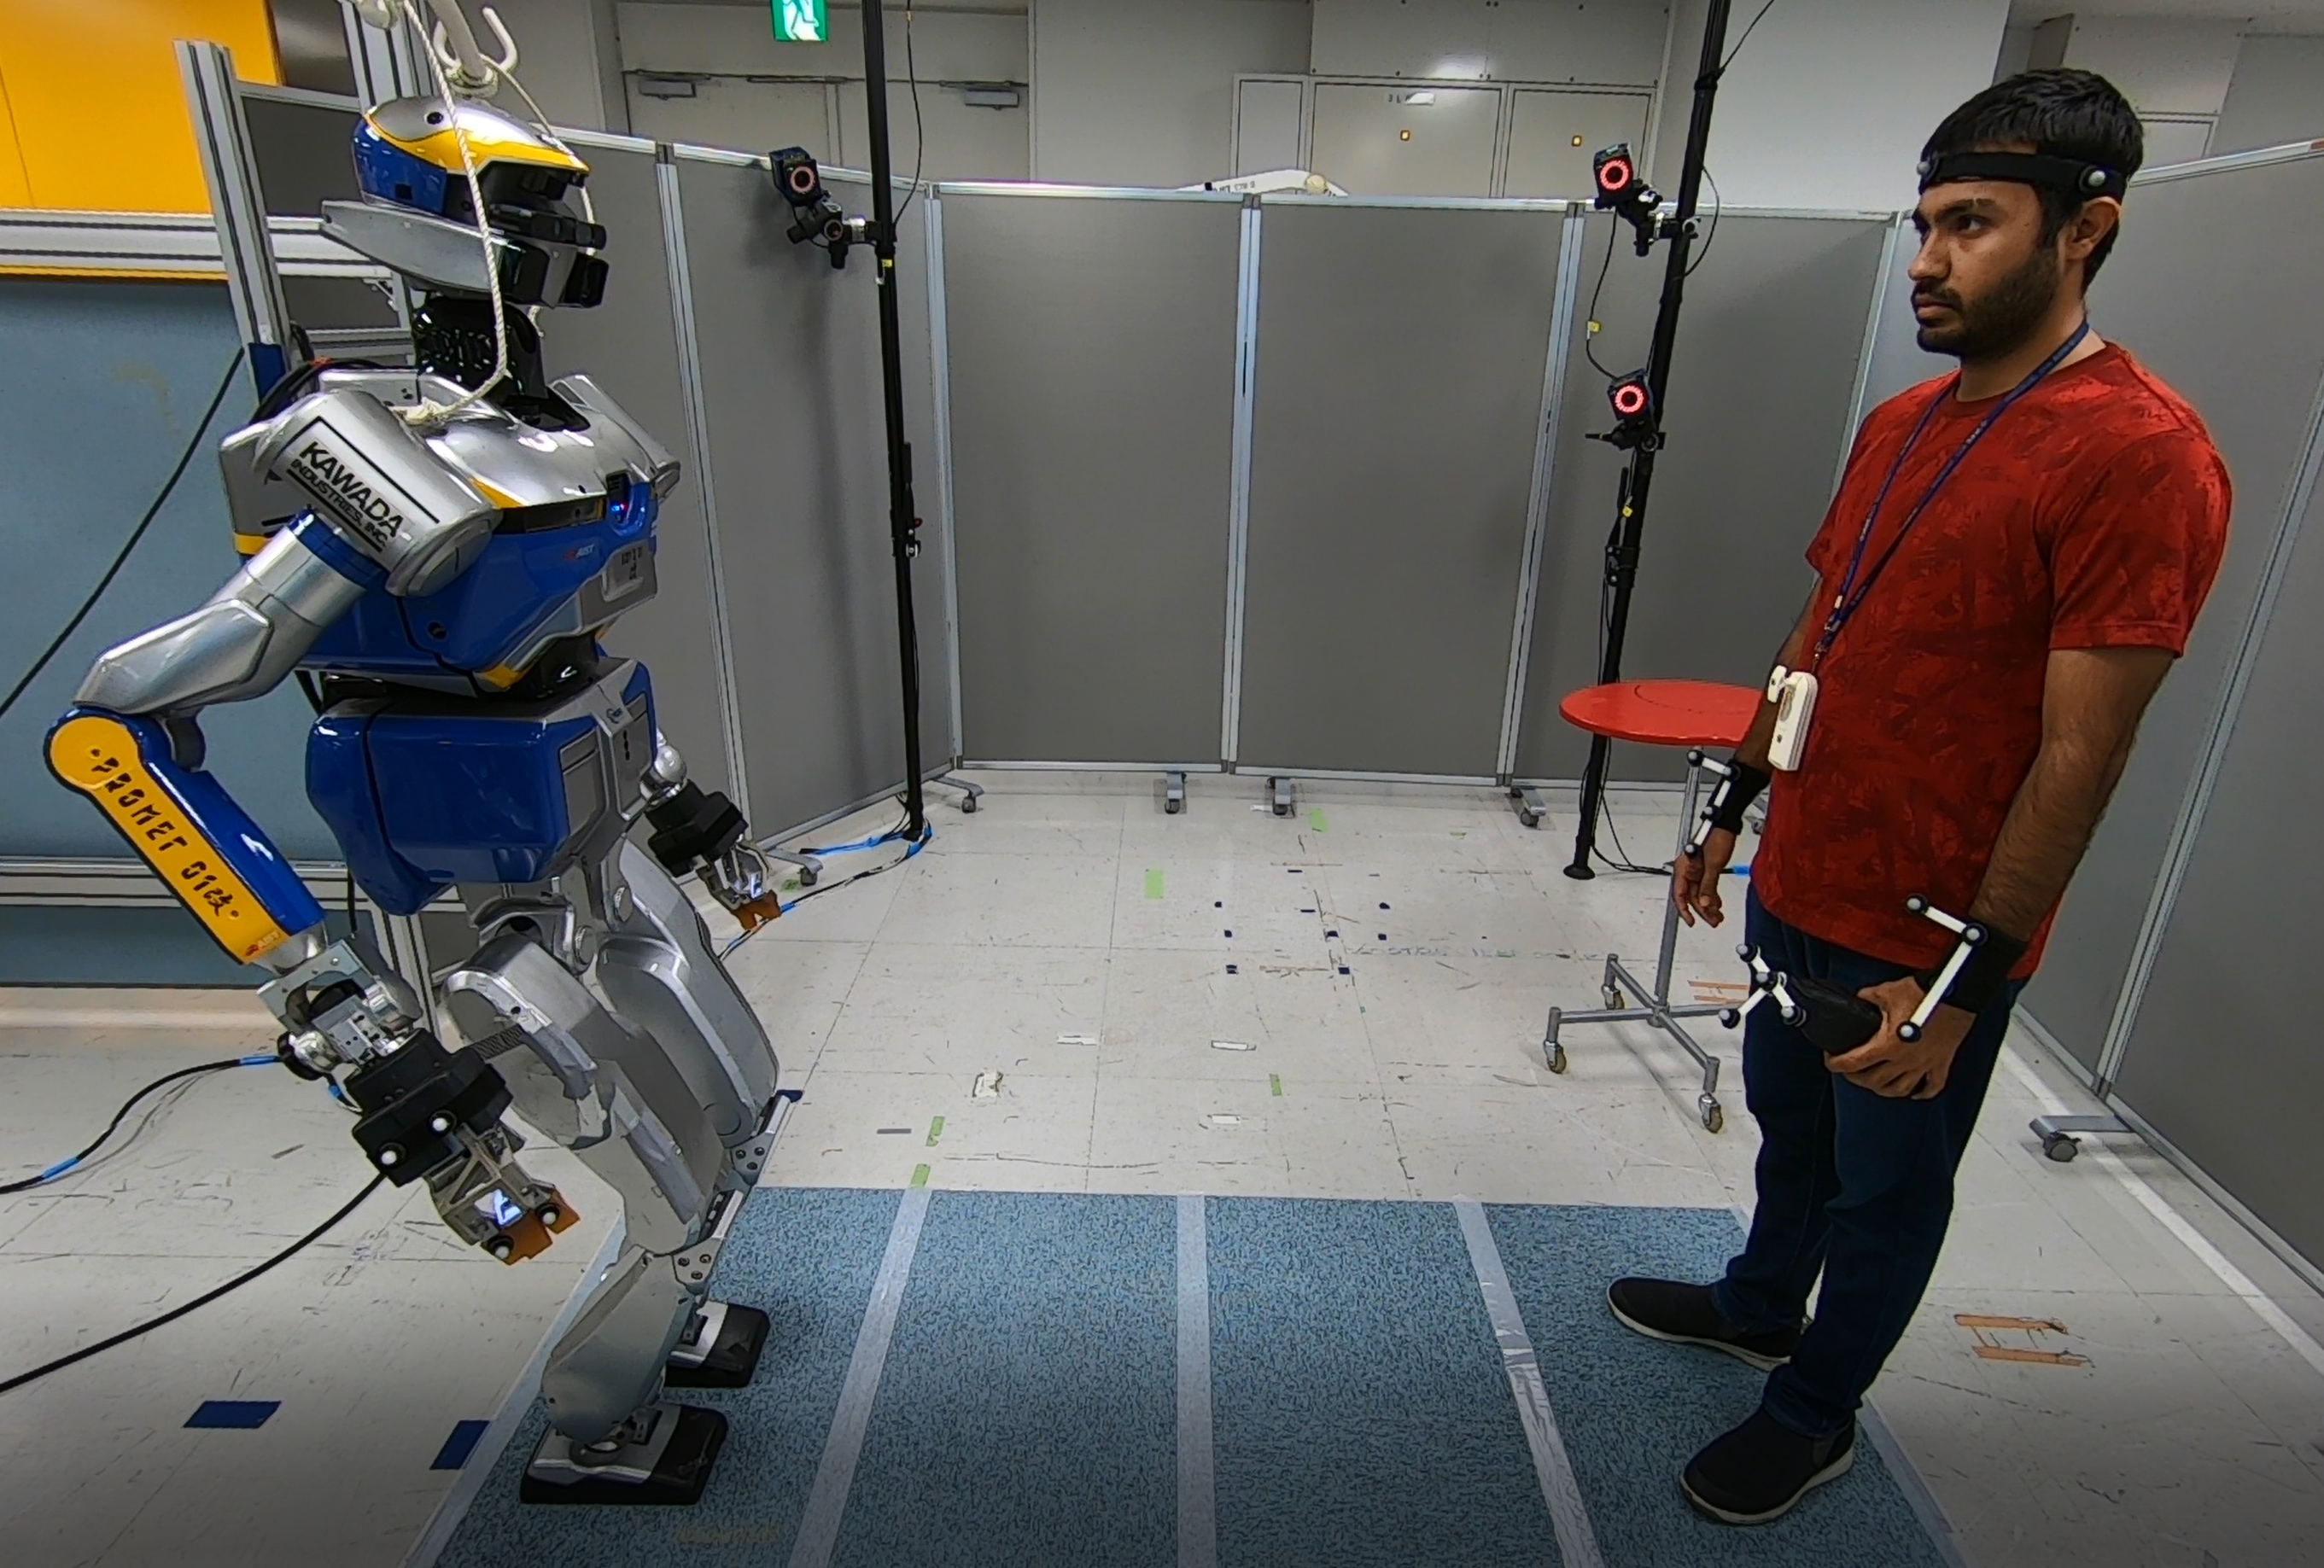
\includegraphics[width=1\columnwidth]{plots/c4-plots/halfsit}}
		\caption{Human and humanoid robot starting posture.}
		\label{fig:halfsit}
\end{figure}


We formulate the bi-directional object handover between human and humanoid robot as single action process (namely, a \textit{cycle}) with different human hand poses (positions and orientations) for object handover and return request along with human hand speed and trajectories. Both human and robot always initiate handover from a starting posture (see Fig.~\ref{fig:halfsit}). We assume that human is ready with the intention to handover object to robot if he/she is holding the object in his/her hand. At handover location, robot takes the object that is handed by the human in a single action event (and vice-versa). Human when carrying the object must hand it seriously to the robot. The human carries the object to different handover locations with distinguishable orientations of object carrying hand and tries to give the object to robot. Similarly, during 2$^{nd}$ \textit{cycle} of handover, human approaches somewhere in the robot workspace with an intention to receive the object from robot using his/her choice of hand orientation and handover location. 



In Fig.~\ref{fig:handover routine}, we describe the process of our bi-directional handover routine using a continuous yet step-by-step approach. We started handover routine to handover object using human right hand to robot left end-effector, from hereafter until and before Section~\nameref{both hands individual} we will explain everything under this condition, afterwards we will talk about generalization of handover using possible handover combination scenarios. Such as,

\begin{itemize}
    \item \textbf{human right hand $\longleftrightarrow$ robot left end-effector}
    \item human left hand $\longleftrightarrow$ robot left end-effector 
    \item human left hand $\longleftrightarrow$  robot right end-effector
    \item human right hand $\longleftrightarrow$ robot right end-effector
\end{itemize}


Just like during human to human object handover, another thing that we incorporated in our handover routine is to give visual tracking like behavior to our robot HRP-2Kai by following an object or a human hand depending on the handover \textit{cycle} using robot's head. We utilized our robot's QP controller (see Section~\nameref{QPController}) and defined a QP based gaze task to follow object during 1$^{st}$ \textit{cycle} of handover and human hand carrying object during 2$^{nd}$ \textit{cycle} of handover.

\begin{figure}[htp]
	\centering
	\tikzstyle{line} = [draw, -latex']
		
	\tikzstyle{cloud} = [draw, ellipse,fill=blue!20, text width=6em, text centered, node distance=4cm,  inner sep=0pt, minimum height=2em]
	
	\tikzstyle{startstop} = [rectangle, text centered, rounded corners, minimum width=3cm, minimum height=1cm, draw=black, node distance=4cm, fill=red!30]

	\tikzstyle{io} = [trapezium, trapezium left angle=70, trapezium right angle=-70,text centered, text width = 1cm,minimum height=1cm, minimum width=2cm, node distance=4cm, draw=black, fill=blue!30]
	
	\tikzstyle{process} = [rectangle, text centered, minimum width=1cm, minimum height=1cm, draw=black, fill=orange!30]

	\tikzstyle{block} = [rectangle, draw, fill=green!20, text width=10em, text centered, node distance=4cm, minimum height=4em]
	
	\tikzstyle{decision} = [diamond, draw, fill=yellow!20, text width=6em, text badly centered, node distance=4cm, inner sep=0pt]

	\begin{tikzpicture}[node distance = 3cm, auto]
		
	\node [process] (or) {1$^{st}$ or 2$^{st}$ \textit{cycle}};

	\node [startstop, above of=or, node distance = 2cm, auto] (start) {start handover routine};	
	
	\node [cloud, left of=or] (subj) {human has object};
	\node [cloud, right of=or] (robot) {robot has object};
	
	\node [block, below of=or, node distance=2cm] (init) {initialize prediction model};
	\node [io, left of=init] (in1) {robot Ef pose};
	\node [io, right of=init] (in2) {human hand pose};
	
	\node [block, below of=init, node distance = 3cm, auto] (relativePos) {observe human hand pose relative to robot Ef pose};
	
	\node [decision, below of=relativePos] (within) {has human hand arrived within robot constraint workspace?};
	\node [block, left of=within, node distance=5cm, text width=5em] (wait) {wait \& head-track human hand};
	\node [block, below of=within, node distance=4cm] (moveEf) {start moving robot Ef to predicted position};
	
	\node [decision, below of=moveEf, node distance = 4cm] (ifClose) {is human hand close enough to robot?};
	\node [startstop, below of=ifClose, node distance=3cm] (event) {handover object};
	
	% Draw edges
	\path [line] (subj) -- (or);
	\path [line] (robot) -- (or);
	\path [line] (start) -- (or);
	\path [line] (or) -- (init);
	
	\path [line,dashed] (in1) -- (init);
	\path [line,dashed] (in2) -- (init);
	\path [line] (init) --  node {FSM} (relativePos);
	\path [line] (relativePos) -- (within);

	\path [line] (wait) |- (relativePos);
	\path [line] (within) -- node [near start] {no} (wait);
	\path [line] (within) -- node {yes} (moveEf);
	
	\path[line] (moveEf) -- (ifClose);
	\path [line] (ifClose) -- node [near start] {no} (moveEf);
	\path [line] (ifClose) -- node [near start] {yes} (event);
	
	\end{tikzpicture}
	
	\caption{Overview of human humanoid robot bi-directional handover routine.}
	\label{fig:handover routine}
\end{figure}

\clearpage

\section{Experimental setup}
We chose our AIST-CNRS-Joint Robotics Laboratory in Tsukuba Japan as the environment to perform our handover routine between human and humanoid robot co-worker. Our experiment setup is shown in Fig.~\ref{fig:halfsit}. Initially we start by having human (participant) and robot co-worker standing comfortably in front of each other at a distance of 1.2 meters from each other. We have always started handover \textit{cycle} by handing over object from human to robot co-worker. The object that needs to be handover was initially either presented to human participant by the experimenter or were kept on the table next to participant, ready to be grasped by him/her. We assume that human participant is ready with the intention to handover object to robot if he/she is holding the object in his/her hand. The whole setup was partially enclosed by movable panels as we didn't wish to perform this experiment under total isolation.


\subsection{Robot}
We used an HRP-2Kai robot~\cite{Kaneko:RAS_ICHR:2015} as the robot co-worker which has  h two arms and legs, a head and a torso. HRP-2Kai is a life-size biped humanoid robot which is 154cm tall, has 32 degree-of-freedoms and weighs about 58kg. It is designed and manufactured by Kawada Industries, Inc in collaboration with AIST under Humanoid Robotics Project (HRP). Both co-workers used their both hands/end-effectors in the experiment.


\subsection{Mocap}
We used motion capture (in short \textit{mocap}) system manufactured by ({\it Motion Analysis Co.,}), to track and get position data of passive reflective markers. We used in total fifteen to seventeen passive reflective markers during several handover scenarios. These markers were placed on the end-effectors of robot co-worker, hands of the participant and on the object itself. These passive markers were tracked using 10 kestrel infra-red cameras, each at 200Hz. These mocap markers position data was later utilized using a real-time interface between mocap system (\texttt{cortex}) and \texttt{ROS} called \textit{ros-cortex-bridge}, which was designed to stream and feed these position data to robot controller in real-time (more information on this can be found in Appendix~\ref{handover appendix}). The markers on the human hand and object were utilized to get their respective position and orientation in the mocap frame and makers on the robot end-effector were used during object handover and release-return of object from robot grippers to human participant as a substitute due to lack of haptic feedback, see Section~\nameref{interaction model} for more details.

\subsection{Handover object(s)}

As shown in Fig.~\ref{fig:objects}, we used three easily distinguishable objects during handover between human and humanoid robot co-worker. We chose these objects because they have different physical structure and mass. These object's mass ranges from $0.22$ kg to $1.1$ kg.


\begin{figure}[htpb]
	\centering{\includegraphics[width=0.8\columnwidth]{plots/c4-plots/objects}}
	\caption{Distinguishable shape and mass objects used during single hand handover between human and humanoid robot co-worker.}
	\label{fig:objects}
\end{figure}


\clearpage

\section{Robot QP controller}\label{QPController}

We used a multi objective Quadratic Programming (QP) based low-level controller, previously designed in our group~\cite{ladder-HRP-2Kai}, to operate and control HRP-2Kai robot behavior. In order to realize human humanoid robot bi-directional object/tool handover study, we introduced several tasks and formulate them in a quadratic fashion so it is conform with QP based controller. The QP enables whole-body control of our HRP2-Kai humanoid robot while respecting internal constraints. To name a few such constraints encompass joints limits, force and torque limits, contact constraints, stability constraints such as keeping center of mass (CoM) inside the support polygon along with self collision constraints and with the environment itself while generating optimal joint trajectories. Some major constraints that robot must satisfy at each time step during human robot object handover are mentioned below.


\subsection{QP constraints}\label{QPConstraints}
The QP controller's objective is to compute an acceleration $\ddot{q}$, where $q$ is the robot configuration vector at each time step $dt$, so as to achieve a set of targets or tasks. The double integration of desired acceleration act as input to built-in PD control of HRP-2Kai. At each $dt$, the QP is formulated and solved by the LSSOL~\cite{gill1986fortran} solver. The tasks are formulated either linear constraints or quadratic costs~\cite{ladder-HRP-2Kai, pfeiffer2017nut}. However, we want to solve these tasks in best possible manner as linearization of some tasks may not be feasible or may be conflicting, therefore using least-square approximation, the quadratic cost $c$ corresponding to task $\mathscr{T}_i =0$ is given by:

\begin{equation}
c_i(q,\dot{q}, \ddot{q})  = \frac{1}{2}{\norm{ J_i\ddot{q} + \dot{J}_i\dot{q} -\ddot{\mathscr{T}}_i }^2 }
\end{equation}

where $J_i$ the Jacobian matrix of $\mathscr{T}_i$, and the QP controller writes following quadratic objective function,

\begin{equation}\label{qp equation}
\min_{\ddot{q},\tau,f} \; \sum_{i\in O} \omega_i c_i(q,\dot{q},\ddot{q}) + \omega_{f}\lVert f\rVert^2
\end{equation}

subject to constraint on equation of motion, as well as other below mentioned constraints,

\begin{equation}
	M(q)\ddot{q} + N(q,\dot{q}) =  J_c^T f
\end{equation}

where $f$ is the set of contact forces, $M$ denotes inertial matrix of the robot, $N$ accounts for Coriolis  and gravity effects, $J_c$ is the Jacobian matrix of all points of contact. The QP objective function in equation (\ref{qp equation}) is made of two terms and the tasks $\mathscr{T}_i$ mentioned in Subsection~\nameref{QPTasks} are weighted against each other by weight $w_i$ based on their relative importance and priority. While the damping weight $w_f$ ensures the smoothness and uniqueness of solution by keeping Hessian matrix positive definite.

\begin{enumerate}	
	\item Static equilibrium:

	$\underline{\tau} \leq J^i(q_i)^Tf_i - g^i(q_i) \leq \overline{\tau}$
	
	where sub-script or super-script $i$ is the $i$-th robot, $q_i$ is the $i$-th robot configuration vector, $f_i$ is the set of contact forces vector of $i$-th robot, $J$ is the Jacobian matrix of all points of contact forces, and $\overline{\tau}$ and $\underline{\tau}$ are the maximum and minimum steady state torque limits respectively, and g be the gravity constant.
	
	\item Joint limits:
	
	$\underline{q_i} \leq q_i \leq \overline{q_i}$
	
	$\underline{q_i}$ and $\overline{q_i}$ are the lower and upper limits for robot joints.
	
	\item Self collisions:
	
	$\delta(X^i_j(q_i), X^i_k(q_i)) > \epsilon_{jk} \qquad \forall(j,k)\in {\mathscr{I}}^i_{self\; collision}$
	
	$\delta$ is the function of distance, $X^i_n(q_i)$ is the occupied volume by $n$-th body of robot in configuration $q_i$, $\epsilon_{jk}$ is the pair of user select minimum distances($j$,$k$) and ${\mathscr{I}}^i_{self\;collision}$ is the robot sets of self collision pairs.
	
	\item Environment collision:
	
	$\delta(X^i_j(q_i), X_k) > \epsilon_{jk} \qquad \forall(j,k)\in {\mathscr{I}}^i_{robot\;environment}$
	
	${\mathscr{I}}^i_{robot\;environment}$ is the set of robot environment (object) collision pairs.
	
%	\item acceleration Constraint: $\mathscr{I}_{contact} = J_i(q)\ddot{q}_{s(k)} + \dot{J}(q)_i\dot{q}_{p(k)} = 0$\\
	\item Contact Constraint: $\mathscr{I}_{contact} = J_i(q) (\dot{q}_{s(k)} - \dot{q}_{p(k)}) = 0$\\
	The objective of this constraint is to maintain a null velocity~\cite{ohwovoriole1980externsion} between the joints of bodies in contact, where $p(k)$ and $s(k)$ are the predecessor and successor bodies of robot(s) in contact that imposes a constraint~\cite{featherstone2014rigid}.
\end{enumerate}



\subsection{QP tasks}\label{QPTasks}
As mentioned earlier, we introduced below following outlined tasks to the multi-objective QP controller to achieve safe and reliable human robot object handover. Let function $\mathscr{T}_i(q)$ denote the geometric objectives (task error) that we require to regulate to zero or maintain above zero, i.e. $\mathscr{T}_i(q) = 0$ and $\mathscr{T}_i(q) \geq 0$.  

\begin{enumerate}[start=1,label={\bf\arabic*.}]

\item Posture task: $\mathscr{T}_{posture} = q_d - q = 0$  

\item Com task: $\mathscr{T}_{CoM} = CoM_d - CoM(q) = 0$

\item Joint limit task: $\mathscr{T}_{jlim} = \underline{q_i} \leq q_i \leq \overline{q_i}$  

\item Position task at body $k$: $\mathscr{T}_{pos} = r^d_k - r_k(q) = 0$\\
Where, $r_k$ and $r^d_k$ are the current and desired position of $i$-th robot $k$-th body. Robot end-effector position task is used to reach the desired handover location~\cite{ladder-HRP-2Kai}.

\item Orientation task at body $k$: $\mathscr{T}_{ori} = Err((E^d_k),  E_k(q))$\\
Where, $E_k$ is the orientation of $i$-th robot body to world. Robot end-effector orientation task is used to compute orientation relative to human hand orientation.

\item Gaze task : $\mathscr{T}_{gaze} =u_{target} - u = 0$\\
Where, $u_{target}$  and $u$ are the target vector in world and body vector that needs to be orient respectively. We used gaze task to orient the head joints of HRP-2Kai towards the active human hand position in world, more details can be found in~\cite{samy2017VecOriTask}.

\end{enumerate}


\clearpage

\section{Notations and terminology}
Let $\mathcal{M}$ (Mocap) and $\mathcal{R}$ (Robot) be the two fixed frames with same orientation that denote both Cartesian coordinate systems and Pl\"ucker coordinate systems denoted by $X$ in the Euclidean space. Both $\mathcal{M}$ and $\mathcal{R}$ are defined by their position and orientation of a Cartesian frame, such that ${}^MX_R$ denotes the Pl\"ucker coordinate transform which depends only on the position and orientation of frame $\mathcal{M}$ relative to frame $\mathcal{R}$ (see Fig~\ref{fig:frames}).

\begin{figure}[ht]
	\centering{\includegraphics[width=0.5\columnwidth]{plots/c4-plots/frame}}
	\caption{$\mathcal{M}$ and $\mathcal{R}$ Cartesian coordinate systems.}
	\label{fig:frames}
\end{figure}


\begin{itemize}
	\item The mathematical notations in the following sections follows ISO guidelines. The Euclidean distance is represented in meters and angles are represented in degrees. The time unit is set in seconds or mentioned otherwise.
	
	\item We used 6D spatial vectors to express the pose of human hand and robot end-effector as well as object. We therefore adopt a 6D notation based on spatial vectors, which is explained in Chapter 2 of~\cite{featherstone2014rigid}.
	
	\item Using QP \texttt{Orientation} task and \texttt{Position} task (see Subsection~\nameref{QPTasks}), we get robot end-effector current orientation ${{}^{ef}\mathcal{O}_R} \in \mathbb{R}^{3\times3}$ and current position ${{}^{ef}\mathcal{P}_R} \in \mathbb{R}^{3}$ respectively in the $\mathcal{R}$ frame, therefore,
	\begin{gather}\label{X_R_ef}
	{}^{ef}{X}_R =
	\left[\begin{array}{cc}
	{}^{ef}\mathcal{O}_R & {}^{ef}\mathcal{P}_R
	\end{array}\right]
	\end{gather}
	
	\item Likewise, ${{}^{h}\mathcal{O}_M} \in \mathbb{R}^{3\times3}$ and ${{}^{h}\mathcal{P}_M} \in \mathbb{R}^{3}$, denotes the human hand $h$ orientation and position respectively in the $\mathcal{M}$ frame, obtained from the $\mathcal{L}$ shape body (see Section~\nameref{hand_orientation}),
	\begin{gather}\label{X_M_h}
	{}^{h}{X}_M =
	\left[\begin{array}{cc}
	{}^{h}\mathcal{O}_M & {}^{h}\mathcal{P}_M \\
	\end{array}\right]
	\end{gather}
	
	\item ${{}^{h}\mathcal{O}_{ef}} \in \mathbb{R}^{3\times3}$ and ${{}^{h}\mathcal{P}_{ef}} \in \mathbb{R}^{3}$ respectively, denotes the human hand $h$ orientation and position relative to robot end-effector,
	\begin{gather}\label{X_ef_h}
	{}^{h}{X}_{ef} =
	\left[\begin{array}{cc}
	{}^{h}\mathcal{O}_{ef} & {}^{h}\mathcal{P}_{ef} \\
	\end{array}\right]
	\end{gather}
	
	\item For convenience, we formulate the problem with a common origin {\it O}, such that $\mathcal R \equiv M$ (both frames are located between the feet of robot HRP-2Kai), we can get human hand pose $\mathsf{w.r.t.}$ or relative to robot end-effector
	
	\begin{equation}\label{X_ef_h1}
	{}^{h}{X}_{ef} = {}^{h}{X}_{M}  {}^{ef}{X_{R}}^{-1}
	\end{equation}
	\item otherwise, when $\mathcal R \neq M$
	
	\begin{equation}\label{X_ef_h2}
	{}^{h}{X}_{ef} = {}^{h}{X}_{M}  {}^{M}{X}_R  {}^{ef}{X_{R}}^{-1}
	\end{equation}
	
\end{itemize}

\clearpage

\section{Human hand orientation model}\label{hand_orientation}
To get the orientation of human hand, we placed a rigid body with a shape similar to an alphabet $L$ on wrist of human hand(s) as shown in Fig~\ref{fig:lshapes}. The three mocap markers $A, B$ and $C$ make up the three vertices of $\mathcal{L}$ shape body, such that during object handover scenario, vector $\vec{AB}^{\,}$ along the longer side and vector $\vec{BC}^{\,}$ along the shorter side are set to be parallel with the $X$-axis and $Y$-axis of the mocap frame $\mathcal{M}$ respectively. The vectors $\vec{AB}^{\,}$ and $\vec{BC}^{\,}$ are orthogonal to each other. For simplicity, let $\hat{x}$ be the unit vector, which is parallel and along the $X$-axis and likewise, unit vector $\hat{y}$ is parallel and along the $Y$-axis of the mocap frame $\mathcal{M}$, such that

\begin{figure}[ht]
	\centering{\includegraphics[width=1\columnwidth]{plots/c4-plots/lshpe-lt-rt}}
	\caption{$\mathcal{L}$ shape rigid body on the human hand(s)}
	\label{fig:lshapes}
\end{figure}

\begin{equation*}
\hat{x} = \frac{\vec{AB}^{\,}}{\norm{\vec{AB}^{\,}}}
\end{equation*}

\begin{equation*}
\hat{y} = \frac{\vec{BC}^{\,}}{\norm{\vec{BC}^{\,}}}
\end{equation*}


Let ${}^{h}\mathcal{O}_{M}$ in equation (\ref{X_M_h}) be the column rotation matrix representing the human hand orientation in the mocap frame $\mathcal{M}$ and since $\hat{x} \in \mathbb{R}^{3}$ and $\hat{y} \in \mathbb{R}^{3}$ are the two orthogonal unit vectors of an $\mathcal{L}$ shape rigid body on human's each hand (Fig~\ref{fig:lshapes}), the cross product of them would result in another unit vector $\hat{z} \in \mathbb{R}^{3}$ which is orthogonal to both $\hat{x}$ and $\hat{y}$. The direction of the cross product would be given by equation (\ref{cross}) using right-hand rule.


\begin{equation}\label{cross}
\hat{z} = \hat{x} \times \hat{y}
\end{equation}



To get the orientation of human hand we used these unit vectors $\hat{x}, \hat{y}$ and $\hat{z}$ as columns of the rotation matrix~\cite{evans2001rotations, altmann2005rotations, jia2017rotation} ${}^{h}\mathcal{O}_{M}$ in equation (\ref{rotationmatrix}), such that the unit vectors $\hat{x}, \hat{y}$ and $\hat{z}$ represents human hand orientation around the $roll-pitch-yaw$ axes respectively.

\begin{equation}\label{rotationmatrix}
{}^{h}\mathcal{O}_{M} = 
\left\{\begin{array}{cccc}
\hat{x.x} & \hat{y.x} & \hat{z.x} \\
\hat{x.y} & \hat{y.y} & \hat{z.y} \\
\hat{x.z} & \hat{y.z} & \hat{z.z}
\end{array}\right\}_{3\times 3}
\end{equation}



\clearpage

\section{Human hand position prediction model}\label{prediction_model}
Algorithm (\ref{positionalgo}) explains the procedure of predicting human hand position and estimating handover location. Inputs to the prediction model are robot left end-effector pose $\mathcal{}^{ef}{X}_R$ (eq~\ref{X_R_ef}) in the robot frame and human hand mocap markers positions ${}^{h}\mathcal{P}_M$ (eq~\ref{X_M_h}) in the mocap frame of reference.


Note that for simplicity, we formulated the problem with a common origin {\it O}, such that frame $\mathcal R \equiv M$, also from onwards by ${}^{h}\mathcal{P}_M$ we meant position of the point $A$ on the $\mathcal{L}$ shape body as the human hand marker position as shown in Fig~\ref{fig:lshapes}.



The prediction model behavior can be tuned by two initially required constant time periods, $t_{observe}$ ---a predefined time period required to observe the motion of human hand and $t_{predict}$ ---required to predict the human hand position in advance.


In order for handover between human and humanoid robot HRP-2Kai to be smooth and intuitive, the robot needs to pro-actively estimate the position of handover location in advance during both cases when robot act as receiver or when robot acts as giver, therefore we formulate the motion of human hand as a constant velocity based linear motion model (see Algorithm (\ref{positionalgo})) to predict the handover position continuously. The robot observes human hand for a predefined time period $t_{observe}$ and predicts the human hand direction and position based on the human hand velocity using equations (\ref{predictVel}) and (\ref{predict}) during the predefined time period. 

\begin{equation} \label{predictVel}
{}^{h}\mathcal{\bar{V}}_{M} = \frac{1}{t_{observe}}{\sum_{j=1}^{j=t_{observe}} ({}^{h}\mathcal{P}_{M}(j)-{}^{h}\mathcal{P}_{M}(j-1))/dt }
\end{equation}

where, $dt$ is controller run-time, in our case it is 5ms, see Section~\nameref{QPController}.

\begin{equation} \label{predict}
{}^{h}\mathcal{P}_M(t_{predict}) = {}^{h}\mathcal{\bar{V}}_{M} \cdot t_{predict}  + {}^{h}\mathcal{P}_{M}(t_{observe})
\end{equation}


The prediction model then updates and converges itself over time and in doing so update the robot end-effector position towards the human hand, upon condition if updated position is within the end-effector's constraint/conditioned workspace, see Fig XXX.


Using equations (\ref{rotationmatrix}) and (\ref{predict}) we get the orientation and translation components of ${}^{h}{X}_M$ in (\ref{X_M_h}), and recalling equations (\ref{X_ef_h1}) and (\ref{X_ef_h2}), the updated translation component of pl\"ucker transformation ${}^{h}{X}_{ef}$, which provides the predicted position of human hand with respect to robot end-effector in the robot coordinate system is given by (\ref{X_ef_ht}), the relative orientation component of ${}^{h}{X}_{ef}$ is discussed in next Section~\nameref{relOri}.

\begin{equation}\label{X_ef_ht}
{}^{h}{X}_{ef}(t_{predict}) =  {}^{h}{X}_M  {}^{M}{X}_R {{}^{ef}{X}_R}^{-1}
\end{equation}

where, ${}^{M}{X}_R$ is the Pl\"ucker coordinate transform frame $\mathcal{M}$ relative to frame $\mathcal{R}$, if $\mathcal R \neq M$.


Finally, the handover location is estimated based on the human hand predicted position when the following conditions satisfy (\ref{min_posErr_vel}), that is when the human hand velocity is minimum and robot end-effector is closest to the human hand.

\begin{equation}\label{min_posErr_vel}
\begin{cases}
	\norm{{}^{h}\mathcal{\bar{V}}_{M}}& <= 1e^{-2} \\
	\norm{({}^{h}\mathcal{P}_{ef}(t_{predict}) - {}^{ef}\mathcal{P}_{R})} & <= 1e^{-2}
\end{cases}
\end{equation}

where, ${}^{h}\mathcal{P}_{ef}(t_{predict})$ is the desired position for robot end-effector to reach and ${}^{ef}\mathcal{P}_{R}$ is the actual current position of robot end-effector and also both positions are in same frame.

\subsection{Algorithm: position prediction model}

\begin{algorithm}[H] \label{positionalgo}
	\DontPrintSemicolon
	\SetNoFillComment
	
	\KwInput{$\mathcal{}^{M}{X}_R, {}^{ef}{X}_R, mocapData$}
	\KwOutput{${}^{h}wp_{ef}$ \tcp*{predicted waypoints}  }
	\KwData{Initial require: $t_{observe}=10ms, t_{predict}=100ms, i=dt=5ms$}
	
	
	\textit{$\textbf{i+=dt}$} \tcp*{increments as per controller run-time (dt)}
	
	\If{$(i\%t_{observe})==0$}
	{
		\For{$j = 1 \textrm{ to } t_{observe} $}
		{
			${}^{h}\mathcal{P}_M= \textit{mocapData}.handMarker(i-t_{observe})+j)$	
		}
		
		${}^{h}\mathcal{\bar{V}}_{M} = \frac{1}{t_{observe}}{\sum_{j=1}^{j=t_{observe}} ({}^{h}\mathcal{P}_{M}(j)-{}^{h}\mathcal{P}_{M}(j-1))/dt }$\newline 
		
		\tcc{predict human hand handover position at $t_{predict}$}
		${}^{h}\mathcal{P}_M(t_{predict}) = {}^{h}\mathcal{\bar{V}}_{M} \cdot t_{predict}  + {}^{h}\mathcal{P}_{M}(t_{observe})$ %\newline % \times 0.005
		
		
		${}^{h}{X}_M= \begin{bmatrix} {}^{h}\mathcal{O}_{M} &  {}^{h}\mathcal{P}_M	\end{bmatrix}$ \newline
		
		\tcc{transform handover position relative to robot end-effector}	
		${}^{h}{X}_{ef}(t_{predict}) =  {}^{h}{X}_M  {}^{M}{X}_R {{}^{ef}{X}_R}^{-1}$ \newline
		
		
		\tcc{\textit{way points between human hand and robot end-effector handover location}}
		\SetKwFunction{FMain}{generateWp}
		\SetKwProg{Fn}{Function}{:}{}
		\Fn{\FMain{$ {}^{ef}\mathcal{P}_{R}, {}^{h}\mathcal{P}_{ef}(t_{predict}), t_{predict} $}}
		{
			\For{$k = 0 \textrm{ to } t_{predict} $}
			{
				${}^{h}wp_{ef}(k) = [{}^{h}\mathcal{P}_{ef}(t_{predict}) - {}^{ef}\mathcal{P}_{R}] . (\frac{k}{t_{predict}})  + {}^{ef}\mathcal{P}_{R} $ 
			}	
			\textbf{return} $ {}^{h}wp_{ef} $
		}
	}
	\caption{linear prediction model - Position}
\end{algorithm}


\clearpage

\section{Relative orientation model}\label{relOri}
The translation component of ${}^{ef}{X}_R $ in the equation (\ref{X_R_ef}) is updated based on the predicted position of human hand (see Section~\nameref{prediction_model}) while the orientation component is updated based on the relative orientation of human hand (see Section~\nameref{hand_orientation}).

\begin{figure}[htpb]
	\centering{\includegraphics[width=.7\linewidth]{plots/c4-plots/rviz_robot_lt_hand_obj_frame}}
	\caption{Robot HRP-2Kai (left end-effector) holding object with fixed orientation during handover in the robot frame $\mathcal{R}$}
	\label{fig:robot_lt_hand_obj}
\end{figure} 

\begin{figure}[htpb]
	\centering{\includegraphics[width=.7\linewidth]{plots/c4-plots/rviz_robot_lt_hand_obj-2layer-empty}}
	\caption{Robot HRP-2Kai (left end-effector) fixed orientation during two handover trials in the robot frame $\mathcal{R}$}
	\label{fig:robot_lt_hand_2layers}
\end{figure} 

Since our robot HRP-2Kai lacks conventional anthropomorphic hands, but instead it has gripper alike hands~\cite{kaneko2015humanoid, stasse2019overview} mainly to increase the manipulability. For relative orientation model to work, we were required to know the fixed initial orientation of the robot end-effector, in which object handover is feasible between human and robot HRP-2Kai, irrespective of the human hand orientation, therefore consider a possible  scenario where the robot end-effector orientation is fixed throughout the handover cycle (transfer of object from human to robot and return to human), irrespective of the condition where robot is a giver or receiver. Let ${{}^{efInit}\mathcal{O}_R}$ denote the initial and fixed orientation of the robot end-effector in the robot frame $\mathcal{R}$ during such human robot object handover scenarios as shown in Fig~\ref{fig:robot_lt_hand_obj}, and Fig~\ref{fig:robot_lt_hand_2layers}, where, ${{}^{efInit}\mathcal{O}_R}$ $\subset$ ${{}^{ef}\mathcal{O}_R}$.




In order to correctly transform desired human hand orientation into robot end-effector frame, we further utilize the equation (\ref{X_ef_ht}). We take advantage of the QP's \texttt{Orientation} Task~\cite{murray2017mathematical, ladder-HRP-2Kai} (see Subsection~\nameref{QPTasks}) and compute the task error $Err$ between \textit{current} human hand orientation and \textit{fixed} robot end-effector orientation, the resulting orientation from the \texttt{Orientation} Task is the desired robot end-effector orientation relative to the human hand orientation (see Fig~\ref{fig:robot_lt_orientations} for few of many possible orientations), therefore using fixed orientation component  ${{}^{efInit}\mathcal{O}_R}$, of equation (\ref{X_R_ef}) and current human hand orientation ${}^{h}\mathcal{O}_M$ from equation (\ref{rotationmatrix}) derived in Section~\nameref{hand_orientation}, we further modify equation (\ref{X_ef_ht}) to get the desired orientation $ {}^{h}\mathcal{O}_{ef} $ of robot end-effector to handover the object.

\begin{figure}[ht]
	\centering{\includegraphics[width=1\columnwidth]{plots/c4-plots/robot_lt_orientations}}
	\caption{Robot HRP-2Kai (left end-effector) holding object in multiple possible orientations during handover trials in the robot frame $\mathcal{R}$.}
	\label{fig:robot_lt_orientations}
\end{figure} 


\begin{gather}\label{X_efinit_hori}
\left[\begin{array}{cc}
\bf{{}^{h}\mathcal{O}_{ef}} & {}^{h}\mathcal{P}_{ef}
\end{array}\right] =
\left[\begin{array}{cc}
\bf{{}^{h}\mathcal{O}_M} & {}^{h}\mathcal{P}_M
\end{array}\right]
\left[\begin{array}{cc}
{}^{M}\mathcal{O}_R & {}^{M}\mathcal{P}_R
\end{array}\right]
\left[\begin{array}{cc}
\bf{{}^{efInit}\mathcal{O}_{R}} & {}^{ef}\mathcal{P}_{R}
\end{array}\right]^{-1}
\end{gather}



\clearpage

\section{Handover interaction model}\label{interaction model}

One of the main problem we focused here is related to the \textit{timing} of grasping and releasing the object. The \textit{timing} at which the robot should close its gripper in order to hold the object, if robot tries to close too early to grasp the object when human is not ready it can lead to collision resulting in an accident or if robot waits too long then it just depreciate the purpose of this study. Along with the previously mentioned problem we also address here another issue related with the \textit{magnitude} of interaction forces between human and robot end-effector holding the object during the release of object in the 2$^{nd}$ cycle of handover i.e. when robot returns the object to the human.


We had to find the equilibrium for robot to know the appropriate \textit{timing} at which the handover should occur, which would be natural and intuitive to the eyes of human, keeping in mind that HRP-2Kai doesn't have anthropomorphic hands but rather manipulative grippers and at the same time we needed to come up with a solution to keep the \textit{magnitude} of interaction forces at minimum. We came up with two methods to tackle this problem, one highlights simplicity and other highlights efficiency but when used together we get a reliable and safest solution possible under such scenario.


HRP-2Kai is equipped with 6-axis \textit{wrist} force sensor on both hands, capable of precisely sensing interaction forces and torques with the environment along $x, y, z$ axes of the sensor local coordinate frame (let's call it $s$). We designed a model of interaction forces which enable the robot end-effector to interact with the object independent of the knowledge of object's mass in advance.

\subsection{Method 1: mocap marker based}
Without actual haptic sensor feedback information from the robot end-effector, we had to rely on the wrist force sensor and mocap markers data of the robot end-effector(see Fig.~\ref{fig:markerEf}), therefore we used mocap makers in conjunction with the force feedback from the wrist sensor of HRP-2Kai robot to know whether the object is within its vicinity to grasp or not. Mocap makers on the robot end-effector were crucial to know the relative position of object from the human hand holding it and the humanoid robot end-effector(s). We placed four passive infra-red markers on the robot end-effector(s) in rectangular shape configuration as shown in Fig.~\ref{fig:markerEf2}. Two of the markers were placed parallel and along the local $x$-axis of force sensor on the wrist of robot end-effector and rest two markers were placed on the gripper tips as shown in Fig.~\ref{fig:markerEf}.

\begin{figure}[ht]
	\centering{\includegraphics[width=.5\linewidth]{plots/c4-plots/markerEf.jpg}}
	\caption{Passive IR markers on the robot HRP-2Kai right end-effector.}
	\label{fig:markerEf}
\end{figure} 


Let \{${}^{wa}\vec P, {}^{wb}\vec P, {}^{ga}\vec P, {}^{gb}\vec P$\} $\in \mathbb{R}^{3}$ be the four position vectors of the mocap markers that are placed on the robot end-effector wrist and gripper tips respectively, also let ${}^{obj}\vec P\in \mathbb{R}^{3}$ be the position vector of mocap marker that placed on the object as shown in the Figures~\ref{fig:robot_lt_hand_obj} and~\ref{fig:robot_lt_orientations}. To get the relative position of object and human hand with respect to robot end-effector, assuming human has the object and is ready with the intent to handover the object. We utilized basic linear algebra and vector products~\cite{brand1947vector, crowe1994history, artin2016geometric} to get the area of triangles $\triangle{{}^{wa}P {}^{wb}P {}^{ga}P}$, $\triangle{{}^{wa}P {}^{wb}P {}^{gb}P}$ and $\triangle{{}^{wa}P {}^{wb}P {}^{obj}P}$ using equation (\ref{area general}) such that upon the satisfaction of following conditions in equation (\ref{area bool}) would give us the relative position of object. Basically we were interested in the output of function $f({}^{obj}\vec{P})$, positive output means that object is within the graspable reach of robot end-effector and that the robot now is ready to close the gripper.

% https://math.stackexchange.com/questions/738236/how-to-calculate-the-area-of-a-triangle-abc-when-given-three-position-vectors-az

\begin{equation}\label{area general}
        \triangle{ABC} = \frac{\norm{ \vec{AB} \times \vec{AC} }} {2} \\
\end{equation}
where $\vec{A}$, $\vec{B}$, $\vec{C}$ are the three coordinate vectors of a triangle $\triangle{ABC}$,


\begin{equation}\label{area}
    \centering
    f({}^{obj}\vec{P}) = 
    \begin{cases}
     (\triangle{{}^{wa}P {}^{wb}P {}^{ga}P} - \triangle{{}^{wa}P {}^{wb}P {}^{obj}P}) > 0 \quad \bigwedge \\
     (\triangle{{}^{wa}P {}^{wb}P {}^{gb}P} - \triangle{{}^{wa}P {}^{wb}P {}^{obj}P}) > 0
   \end{cases}         
\end{equation}

\begin{equation}\label{area bool}
    \centering
    if
    \begin{cases}
     f({}^{obj}\vec{P})==1, & \text{within graspable reach}  \\
     f({}^{obj}\vec{P})==0, & \text{object outside gripper}
   \end{cases}         
\end{equation}





\begin{figure}[ht]
	\centering{\includegraphics[width=\linewidth]{plots/c4-plots/efmarkers.png}}
	\caption{Passive IR markers on the robot HRP-2Kai right end-effector, human left hand and object during handover.}
	\label{fig:markerEf2}
\end{figure} 

We explained further in detail in the Subsection~\nameref{FSM}, but before that we mention another~\nameref{surface wrench} that we also utilize for closing gripper when object is in the vicinity.



\subsection{Method 2: surface wrench based}\label{surface wrench}

\begin{figure}[ht]
	\centering{\includegraphics[width=0.8\columnwidth]{plots/c4-plots/wrist-surface2}}
	\caption{Virtual intrinsic surfaces (green) on robot wrists.}
	\label{fig:wrist-surface2}
\end{figure}

Just by knowing the relative position of the object with respect to the robot end-effector gripper is not enough for safe and reliable object handover. This is due to the lack of anthropomorphic hands and the visual features of the manipulative gripper can be intimidating to some humans. Therefore in conjunction to the mocap marker based method mentioned earlier we also computed ${}^{surf}\vec{f}$, the \textit{gravity-free} force vector in the intrinsic surface frame $surf$ of the gripper (see Fig.~\ref{fig:wrist-surface2}). Let ${}^s\vec{f}\in F^6$ denote the \textit{gravity-free} spatial force vector in the local sensor frame $s$. Note that ${}^s\vec{f}$ has both force and couple components, but we were only interested in the force component. We can easily get the coordinate transformation between surface frame and force sensor frame, knowing the body at which force sensor is attached.

\begin{equation}\label{X_s_surf}
    {}^{surf}X_{s} = {}^{surf}X_{b} {}^{b}X_s
\end{equation}

where, $b$ denotes the body frame at which the force sensor is attached, in our case force sensors are attached to the wrist of HRP-2Kai. One can generally obtain the transform matrix for a force vector as explained in~\cite{featherstone2014rigid} if $X$ is responsible for coordinate transformation on motion vectors then using the equation (\ref{X*}), $X^{*}$ would do same transformation on force vectors, since both are related~\cite{featherstone2014rigid},

% check page 17-25
\begin{equation}\label{X*}
    X^{*} = X^{-T}
\end{equation}

and therefore, force vector in the surface frame $surf$ can be obtained by utilising equations (\ref{X*}) and (\ref{X_s_surf}), we get

% Dual Coordinates: page 9~\cite{featherstone2014rigid} $X^{*} f$, check page 246 as well
\begin{equation}\label{force surf}
    {}^{surf}\vec{f} = {}^{surf}X_{s}^{*} {}^s\vec{f}
\end{equation}

where, ${}^{surf}X_{s}^{*}$ is the transformation matrix for transformation of force vector from force sensor frame $s$ to gripper intrinsic surface frame $surf$. Finally we measure noise free $\abs{{}^{surf}\vec{f}}$ along the gripper's insertion ($z$)-axis, during the interaction between object and gripper just prior to handover and if the measured $\abs{{}^{surf}\vec{f}}$ is greater than 3N along with the outcome of equation (\ref{area}) then it is safe for robot to close the gripper and hence grasp the object. We further explained complete handover routine utilizing above discussed methods in the next Subsection~\nameref{FSM} on FSM.

\subsection{Finite state machine}\label{FSM}

\begin{figure}[hpt]
	\centering{\includegraphics[width=1\columnwidth]{plots/c4-plots/h-to-r.jpg}}
	\caption{human to humanoid robot object handover, t1 to t8 transition states.}
	\label{fig:h-to-r}
\end{figure}

The whole handover routine is a continuous process but for clarity we have divided it into several transition steps of Finite State Machine (FSM)~\cite{johnson1968automatic}, also see Fig.~\ref{fig:fsm} for graphical implementation and Algorithm (\ref{interaction forces}) as well, the transitions between states are set to be continuous upon the success of previous transition. In order to understand the interaction forces model, let $\mathcal{\vec{F}}\in \mathbb{R}^3$ denote the current \textit{gravity-free} force sensor reading in the robot frame $\mathcal{R}$. During human to robot handover cycle when human holds the object (see Fig.~\ref{fig:h-to-r}), in such a situation due to any acceleration of the robot end-effector while approaching towards the object, a wrist force sensor would only read inertial forces~\cite{spong2008robot}, which we termed ${}^{zero}\vec{\mathcal{F}}$ as force sensor offset reading (see equation~\ref{Fzero}). Let ${}^{obj}\overline{\mathcal{F}}\in \mathbb{R}^3$ be the average of contact forces between the end-effector (gripper) and the environment (object) during the resting (${}^{ef}v=0$) period of robot end-effector along the $xyz$ axes and let ${}^{inert}\vec{\mathcal{F}}$ be the inertial force acting on the object due to the acceleration (lets call it ${}^{ef}a$) of robot end-effector when moving towards the predicted pose of human hand during the 2$^{nd}$ cycle of handover as shown in Fig.~\ref{fig:r-to-h}. Let ${}^{pull}\vec{\mathcal{F}}$ be the current \textit{minimum} interaction force exerted on the object and sensed by the robot wrist force sensor while retreating the object during robot to human handover cycle and let ${}^{old}T$, ${}^{new}T$ $\in \mathbb{R}^3$ be the respective initial default hand-tuned and updated force thresholds. We now explain each state of FSM as shown in Fig.~\ref{fig:fsm}.

%\footnote{\label{appendixC} To get more information on how we transformed force sensor local frame $s$ into robot world frame $\mathcal{R}$ and without gravity free reading please see Appendix~\ref{handover appendix}.}


\begin{figure}[hptb]
	\centering
	\begin{tikzpicture}[node distance=5cm, auto, scale = 1, ->,>=stealth, line width=2.3pt, kant/.style={text width=2cm, text centered, sloped}]
	\tikzstyle{cloud} = [draw,ultra thick, circle ,fill=white!20, text width=4em, text centered, node distance=9em, auto, inner sep=0pt, minimum height=1em]
	\tikzstyle{blank} = [circle ,fill=white!20, text width=5em, text centered, node distance=5em, auto, inner sep=0pt, minimum height=2em]
	\tikzstyle{line} = [draw, -latex', inner sep=0pt, minimum height=2em]
	
	\node[cloud,initial above] (human has object) {human has object?};
	\node[cloud, node distance=4cm] (human hand is near?) [right of=human has object] {is object near robot?};
	\node[cloud] (open gripper) [below of=human hand is near?] {open gripper};
	\node[cloud] (stop motion) [right of=open gripper] {maintain current pose};
	\node[cloud] (object inside gripper?) [below of=open gripper] {object inside gripper?};
	\node[cloud] (close gripper) [right of=object inside gripper?] {close gripper};
	\node[cloud] (robot has object) [right of=close gripper] {robot receives object};		
	\node[cloud] (go rest pose) [below of=robot has object] {go to rest pose};
	\node[cloud] (start motion) [left of=go rest pose] {continue motion};
	\node[cloud, node distance=3.8cm] (human hand is near again?) [left of=start motion] {human hand near object?};	
	\node[cloud] (pull handover object) [below of=human hand is near again?] {human pulls object?};
	\node[cloud, node distance=5cm] (open gripper release object) [right of=pull handover object] {gripper releases object};
	\node[cloud] (handover occurred) [below of=open gripper release object] {human receives object};
	\node[cloud, node distance=5cm] (go rest pose2) [left of=handover occurred] {go to rest pose};
	\node[blank] (blank)[left of = go rest pose2]{};
	
	\path [line] (human has object) edge     node[above, kant]{t1, 1$^{st}$ cycle} (human hand is near?);
	\path [line] (human hand is near?) edge      node {t2} (open gripper);
	\path [line] (open gripper) edge              node {t3} (stop motion);
	\path [line] (open gripper) edge              node {t4} (object inside gripper?);
	\path [line] (object inside gripper?) edge   node {t5} (close gripper);
	\path [line, dashed] (close gripper) edge          node [above, kant]{t6, if false close?} (open gripper);
	\path [line] (close gripper) edge         node {t7}(robot has object);
	\path [line] (robot has object)edge        node[left]{t8, ${}^{obj}F$} (go rest pose);
	\path [line] (go rest pose) edge           node [above, kant]{t9, 2$^{nd}$ cycle} (start motion);
	\path [line]  (start motion)edge           node [above, kant]{t10, ${}^{inert}F$} (human hand is near again?);
	\path [line]  (human hand is near again?)edge  node {t11, ${}^{pull}F, {}^{new}T$}  (pull handover object);
	\path [line]  (pull handover object)edge       node [below, kant]{t12, ${}^{pull}F >{}^{new}T$} (open gripper release object);
	\path [line]  (open gripper release object)edge  node {t13}(handover occurred);
	\path [line]  (handover occurred)edge           node {t14}(go rest pose2);
	\path [line, dashed]  (go rest pose2) -|       node [near end, above, rotate=90]{t0, \textbf{restart handover}}(human has object);
	
	\end{tikzpicture}
	\caption{Overview of human humanoid robot object handover Finite-State-Machine (FSM)}
	\label{fig:fsm}
\end{figure}


\begin{figure}[hpt]
	\centering{\includegraphics[width=1\columnwidth]{plots/c4-plots/r-to-h.jpg}}
	\caption{humanoid robot to human object handover t9 to t14 transition states.}
	\label{fig:r-to-h}
\end{figure}

\begin{enumerate}[start=0,label={\bf{t}\arabic*:}]
    \item $\norm{{}^h{P} - {}^{obj}{P}} < 0.02$\\
    We start FSM under the assumption that object is already being held by the human and he/she is ready with the intention of handover. ${}^h{P}$ is the position of point $A$ on the $\mathcal{L}$ shape body as the human hand marker position (see Fig.~\ref{fig:lshapes}).
    
    
    \item $\norm{{}^h{P} - {}^{ef}{P}} < 0.10$\\
    1$^{st}$ cycle of handover, i.e. human to robot object handover.\\
    We measure the relative position of human hand and robot end-effector mocap markers, the state transition is successful if the euclidean distance $d$ is less than 0.1 meters, where $d = \norm{{}^h{P} - {}^{ef}{P}}$. ${}^{ef}{P}$ is the average position of gripper tips marker ${}^{ga}P, {}^{gb}P$. 
    
    \item Open Gripper\\
    Robot opens the gripper and presents with its intention to grasp the object.
    
    \item $\norm{{}^h{P} - {}^{ef}{P}} \leq 0.05$, maintain current pose\\
    To avoid collision between robot end-effector and human hand we reduce the end-effector velocity (${}^{ef}v\simeq0$) when the interaction distance $d = \norm{{}^h{P} - {}^{ef}{P}}$ is less than 0.05 meters. We also measure ${}^{zero}\vec{\mathcal{F}}$ as force sensor offset.

    \begin{equation}\label{Fzero}
        {}^{zero}\vec{\mathcal{F}} = \vert{\vec{\mathcal{F}}}
    \end{equation}

    \item ${}^{surf}\vec{f} \geq 3N \quad \bigwedge \quad f({}^{obj}\vec{P})  == 1$\\
    We declare object is inside gripper if output of equations (\ref{area bool},~\ref{force surf}) satisfy together.
    
    \item Close Gripper\\
    Let ${}^{close}\vec{\mathcal{F}}$ be the measured force reading at the timing of closing gripper.
        
        \begin{equation}\label{Fclose}
        {}^{close}\vec{\mathcal{F}} = \vert{\vec{\mathcal{F}}}
        \end{equation}
    
    Robot closes gripper, presumably object is grasped as well. However it is easy to check if the object is really grasped by robot or if its a false close. It is safe to say that its a false close if output of equation (\ref{area bool}) is $0$, along with the condition $\norm{{}^{zero}\vec{\mathcal{F}}-{}^{close}\vec{\mathcal{F}}} \simeq{0}$, since these are same measured force sensor offsets. Therefore, in such scenario next transition would be \textbf{t6} to open gripper and repeat, otherwise \textbf{t7}, as shown in Fig.~\ref{fig:fsm}.
    
    \item Open Gripper, due to false close.
    
    \item This transition confirms that robot receives the object and now the object \textit{mass} can be calculated based on the forces measured during previous states.
    
    \begin{equation}
        {}^{obj}\overline{\mathcal{F}} = \frac{1}{n}\sum_{i=1}^{i=n} \vert{ (\vert{\vec{\mathcal{F}}} - \vert{{}^{zero}\vec{\mathcal{F}}}) }
    \end{equation}
    
    ${}^{obj}\overline{\mathcal{F}}$, is pure force sensor reading when ${}^{ef}a=0$ and object is grasped by the robot, $n$ is the low-level controller time-step counter increments every $5$ms (see Section~\nameref{QPController}), we intentionally stay on this state for 1 second i.e. until $i==200$ to measure average of ${}^{obj}\vec{\mathcal{F}}$ over 200 samples. Object $mass$ can be obtained using equation (\ref{obj mass}).
    
    \begin{equation}\label{obj mass}
        objMass = \norm{{}^{obj}\overline{\mathcal{F}}}/9.81
    \end{equation}

    \item Go to rest pose \\
    Both human and robot returns to their resting posture, with robot carrying the object. End of $1^{st}$ cycle of handover.
    
    \item $2^{nd}$ cycle begins\\
    Robot to human object handover. The robot continues to predict human hand position and moves towards it. During this time we can measure the ${}^{inert}\vec{\mathcal{F}}$ inertial force acting on the object due to end-effector acceleration.

    \begin{equation}
        {}^{inert}\vec{\mathcal{F}}  = objMass * {}^{ef}\overline{a}
    \end{equation}

    Where, ${}^{ef}\overline{a}$, is the average acceleration of the robot end-effector.

    \item $\norm{{}^h{P} - {}^{ef}{P}} < 0.05$\\
    Once again, we measure the relative position of human hand and robot end-effector mocap markers, the state transition is successful if the euclidean distance $d = \norm{{}^h{P} - {}^{ef}{P}}$ is less than 0.05 meters. That means human is ready with the intention to grasp the object.
    
    \item Human attempts to retrieve object
    
    \begin{equation}
    {}^{pull}\vec{\mathcal{F}} = \vert{ (\vert{\vec{\mathcal{F}}} - \vert{{}^{inert}\vec{\mathcal{F}}} - \vert{{}^{zero}\vec{\mathcal{F}}}) }
    \end{equation}
    
    \begin{equation}
    {}^{new}\vec{T} = {}^{obj}\overline{\mathcal{F}} + {}^{old}\vec{T}
    \end{equation}
    
    where, we chose to maintain ${}^{old}\vec{T}$ as default $[5, 5, 5]$ N.
    
    \item Open Gripper, human grasps the object if both below conditions satisfy

    \begin{equation}\label{Fpull}
    \begin{cases}
     \norm{{}^h{P} - {}^{obj}{P}} < 0.02 \quad \bigwedge  \\
     {}^{pull}\vec{\mathcal{F}}\geq {}^{new}\vec{T}, & \lor x, \lor y, \lor z
   \end{cases}
   \end{equation}

    where, $\norm{{}^h{P} - {}^{obj}{P}}$ is again euclidean distance between human hand and object mocap markers.

    \item Object returns to human, human retreats.
    
    \item End of $2^{nd}$ \textit{cycle} of handover.\\
    Both human and robot returns to their resting posture, with human carrying the object.
\end{enumerate}
    
\begin{itemize}
    \item Repeat again handover routine with $1^{st}$ \textit{cycle} of handover.
\end{itemize}

\clearpage

\subsection{Algorithm: interaction forces}
\begin{algorithm}[H]\label{interaction forces}
	\DontPrintSemicolon
	\SetNoFillComment
	
	\KwInput{$\mathcal{F}$\tcp*{EF wrist worldWrenchWithoutGravity}}
	\KwOutput{${}^{pull}\mathcal{F}, {}^{new}T$ \tcp*{Pull force, new threshold based on object mass\newline} }
% 	\textit{$\textbf{dt++}$} \tcp*{increments as per controller run-time (5ms)}
	
	\If{\text{human hand is near robot}}
	{
		\tcc{when human holds the object}
		\If{$\norm{{}^h{P} - {}^{ef}{P}} < 0.10$\tcp*{gripper is empty}}
		{
		    Open Gripper\\
			$\mathcal{}^{zero}{F}= \mathcal{F}$\tcp*{wrench offset}
		}
		\tcc{when robot holds the object}
		${}^{obj}\overline{\mathcal{F}} = \frac{1}{n}\sum_{i=1}^{i=n} \vert{ (\vert{\mathcal{F}} - \vert{{}^{zero}\mathcal{F}}) }$
		
		$objectMass = \norm{{}^{obj}\overline{\mathcal{F}}}/9.81 $\tcp*{get object mass}
		
		${}^{inert}\mathcal{F} = objectMass * efAce$ \tcp*{$efAce$ - end-effector acceleration}
		
		${}^{new}T = {}^{obj}\overline{\mathcal{F}} + {}^{old}T$\tcp*{$T_{old}$ set to [5,5,5]}
		
		\SetKwFunction{FMain}{CheckPullForce}
		\SetKwProg{Fn}{Function}{:}{}
		\Fn{\FMain{$\lor x, \lor y, \lor z$}}
		{	
			${}^{pull}\mathcal{F} = \vert{(\vert\mathcal{{F}} - \vert{}^{inert}\mathcal{{F}} - \vert{}^{zero}\mathcal{{F}}) }$
			
			\If{${}^{pull}\mathcal{F} > {}^{new}T \lor x, \lor y, \lor z$}
			{
				\textrm{release object}\tcp*{release object}
			}
		}
	}
	\caption{Algorithm:Interaction Forces}
\end{algorithm}




\clearpage

\section{Generalized bi-directional handover- \textit{using either hand}}\label{both hands individual}

As mentioned earlier in Subsection~\nameref{handover routine}, up till now we have discussed human robot bi-directional object handover under the scenario where robot always uses its left end-effector and human always uses his/her right hand. However unlike many handover studies in the past [cite XXX XXX XX], we can take the advantage of having a humanoid robot HRP-2Kai at our disposal, therefore we further generalize our human humanoid robot bi-directional object handover routine and extend it by exploiting either human's left or right hand and similarly left or right end-effector of robot. Basically we extended our one-hand handover routine into all four possible scenarios (see Fig.~\ref{fig:handover scenarios}) such as,

\begin{enumerate}
	\item robot left end-effector $R_{efl}$ $\longleftrightarrow$ human right hand $H_r$
	\item robot left end-effector $R_{efl}$ $\longleftrightarrow$ human left hand $H_l$
	\item robot right end-effector $R_{efr}$ $\longleftrightarrow$ human left hand $H_l$
	\item robot right end-effector $R_{efr}$ $\longleftrightarrow$ human right hand $H_r$
\end{enumerate}


\begin{figure}[hpt]
	\centering
	\begin{tikzpicture}[node distance=5cm, auto, scale = 1, ->,>=stealth, line width=2.3pt, kant/.style={text width=2cm, text centered, sloped}]
		\tikzstyle{cloud} = [draw,ultra thick, circle ,fill=white!20, text width=4em, text centered, node distance=9em, auto, inner sep=0pt, minimum height=1em]
		\tikzstyle{line} = [draw, -latex', inner sep=0pt, minimum height=2em]
		
		\node[cloud] (obj) {object};
		\node[cloud] (hl) [below left of = obj] {$H_l$};
		\node[cloud] (hr) [below right of= obj] {$H_r$};

		\node[cloud] (rr) [below of = hl] {$R_{efr}$};
		\node[cloud] (rl) [below of= hr] {$R_{efl}$};

		\path [line] (obj) edge  node[above, kant]{} (hl);
		\path [line] (obj) edge  node[above, kant]{} (hr);		
		
		\path [line] (hl) edge  node[above, kant]{} (rl);
		\path [line] (rl) edge  node[above, kant]{} (hl);
	
		\path [line] (hl) edge  node[above, kant]{} (rr);
		\path [line] (rr) edge  node[above, kant]{} (hl);
	
		\path [line] (hr) edge  node[above, kant]{} (rl);
		\path [line] (rl) edge  node[above, kant]{} (hr);
		
		\path [line] (hr) edge  node[above, kant]{} (rr);
		\path [line] (rr) edge  node[above, kant]{} (hr);

	\end{tikzpicture}
	\caption{Possible handover scenarios between human humanoid robot.}
	\label{fig:handover scenarios}
\end{figure}


In this section we will only mention changes that need to be incorporated into the previous sections for the generalization and extension of previously stated handover routine in Subsection~\nameref{handover routine} to cover above four possible scenarios. We mainly modify here parameters of FSM states during transitions {\bf t0, t1} and {\bf t10}, which are already discussed in detail (see Subsection~\nameref{FSM}). Once again we have assumed that human is ready with the intention to handover the object if he/she is holding it in his/her either hand. We have also assumed that just like humans, our robot also acts like a \textit{right-hand person}, therefore robot right end-effector would get priority over left in case object is at relatively same distance from both end-effectors or in case where the handover predicted position is at or converging towards the center of robot body (cite XXX ganesh given paper). 
%, this is mainly because recent study has shown that right hand human tend to prefer right hand over left


The choice or preference of employing end-effector (either left or right) by the robot is based on the shortest relative distance of object to either human hand using equation (\ref{human obj dist}) along with the direction (mainly along $y$-axis) and shortest relative distance of \textit{that} human hand with respect to both end-effectors, as per equations (\ref{human hand dir} and~\ref{robot obj dis}) respectively. For example, if human is holding object in his/her right hand ${}^{hr}{P}$ and if the estimated predicted position of his/her hand (see Section~\nameref{prediction_model}) is converging somewhere in the negative $y$-coordinate space, then robot right end-effector ${}^{efr}{P}$ would be utilized to receive the object during handover as shown in Fig.~\ref{fig:hr-to-rr}.


\begin{figure}[hpt]
	\centering{\includegraphics[width=1\columnwidth]{plots/c4-plots/hr-rr}}
	\caption{Object handover between human right hand and humanoid robot right end-effector.}
	\label{fig:hr-to-rr}
\end{figure}


\begin{equation}\label{human obj dist}
\centering
\begin{cases}
	\norm{{}^{hl}{P} - {}^{obj}{P}} < \norm{{}^{hr}{P} - {}^{obj}{P}}, & \text{human left hand (${}^{hl}{P}$)}  \\
	\\
	\norm{{}^{hl}{P} - {}^{obj}{P}} > \norm{{}^{hr}{P} - {}^{obj}{P}}, & \text{human right hand (${}^{hr}{P}$)}
\end{cases}         
\end{equation}


\begin{equation}\label{human hand dir}
\centering
\begin{cases}
\norm{{}^{h}{P}(y)} > 0,  &  \text{robot left end-effector (${}^{efl}{P}$)} \\
\\
\norm{{}^{h}{P}(y)} \leq 0,  &  \text{robot right end-effector (${}^{efr}{P}$)}
\end{cases}         
\end{equation}

\begin{equation}\label{robot obj dis}
\centering
\begin{cases}
\norm{{}^{h}{P} - {}^{efl}{P}} < \norm{{}^{h}{P} - {}^{efr}{P}}, &  \text{robot left end-effector (${}^{efl}{P}$)} \\
\\
\norm{{}^{h}{P} - {}^{efl}{P}} > \norm{{}^{h}{P} - {}^{efr}{P}}, &  \text{robot right end-effector (${}^{efr}{P}$)}
\end{cases}
\end{equation}


Where ${}^{h}{P}$ could be either of the human hand position depending upon equation (\ref{human obj dist}), however in cases where there is a switching of object in between human hands and within the same \textit{cycle} of handover such as, human may decide to move the object from his/her left to right hand or vice-versa for any reasons, under those conditions we rely on the effect of \textit{hysteresis} for robot to decide whether it needs to switch end-effector or continue uninterruptedly. Using earlier example where human right hand has the object and his/her position is converging somewhere in the negative $y$-coordinate space while during this cycle of handover if human switches his/her hand in between to hold the object ---say from right to left hand, then by taking recent history (direction) of human hand into account we further utilize the outputs of equations (\ref{human hand dir} and~\ref{robot obj dis}) to measure change in the direction of human hand and its shortest relative distance from the end-effectors, and based on these observations robot decides to act accordingly. By exploiting \textit{hysteresis} effect we make sure that robot doesn't respond abruptly to changes made by human.

%https://en.wikipedia.org/wiki/Hysteresis
%https://arduino.stackexchange.com/questions/9115/how-to-add-hysteresis-to-threshold-values

%In control systems, hysteresis can be used to filter signals so that the output reacts less rapidly than it otherwise would, by taking recent history into account. For example, a thermostat controlling a heater may switch the heater on when the temperature drops below A, but not turn it off until the temperature rises above B. (For instance, if one wishes to maintain a temperature of 20 °C then one might set the thermostat to turn the heater on when the temperature drops to below 18 °C and off when the temperature exceeds 22 °C).

\clearpage

\section{Dual hand bi-directional handover - \textit{using hands together}}\label{both hands together}

It is very natural between humans to use both hands to manipulate a heavy or large shape object to gain confidence and maintain stability during a physical interaction or even while performing a collaborative task. Using both hands together during the course of handing over such object to one another is no different. Similarly, in scenarios where use of single hand is not feasible to perform safe and reliable handover of a heavy large object between human and humanoid robot, then it should be an obvious choice for robot as well to use both hands together whenever necessary. 


We again take the advantage of having a humanoid robot at our disposal and extend the handover routine under the scenario of large object transfer between human and robot. We formulate this handover routine in a manner such that human co-worker is allowed to use either or both hands to handover/receive the object to robot co-worker. However, robot would always use both hands while receiving and returning of such object, given the physical structural properties of the object.

\subsection{Handover object(s)}


\begin{figure}[hpt]
	\centering{\includegraphics[width=1\columnwidth]{plots/c4-plots/handoverPipe}}
	\caption{Hollow cylinder shaft as object for handover between human humanoid robot.}
	\label{fig:pipe_ex}
\end{figure}


The object(s) (two of them) we chose to handover between human and humanoid robot are cylindrical in nature (see Fig.~\ref{fig:pipe_ex}). we chose these objects purely for simplicity and demonstration purposes in this study. Though our handover model would practically work on several distinguishable objects as long as object's basic physical structural properties are known, however mass of object is optional. The cylindrical structures we used are hollow yet quite rigid in nature. The inner $r_i$ and outer $r_o$ radii for those two objects are \textins{$0.055$, $0.065$} m and \textins{$0.07$, $ 0.08$} m respectively, lengths $l$ are \textins{$0.90$, $ 0.12$} m, and the mass of objects are \textins{$0.40$, $1.1$} kg, again we don't need to know mass of object in advance as it can be computed during handover routine when robot carries the object as explained earlier in the Subsection~\nameref{FSM}. 


\begin{figure}[hpt]
	\centering{\includegraphics[width=1\columnwidth]{plots/c4-plots/robot_has_pipe}}
	\caption{HRP-2Kai using both end-effectors to manipulate handover object based on the human hand relative orientation.}
	\label{fig:pipe_ori}
\end{figure}


The object's origin is located at its center as shown in Fig.~\ref{fig:pipe_ex} and Fig.~\ref{fig:pipe_ori} with respective $xyz$ local coordinate axes in local frame $o$ and are along the direction of robot frame axes. The object pose (position and orientation) is given by ${}^{o}{X}_M$. Let ${{}^{o}\mathcal{O}_M} \in \mathbb{R}^{3\times3}$ and ${{}^{o}\mathcal{P}_M} \in \mathbb{R}^{3}$, denotes the object orientation and position respectively in the $\mathcal{M}$ frame, obtained from another $\mathcal{L}$ shape body attached on the object. Object orientation can be formulated similarly to human hand orientation, see Section~\nameref{hand_orientation} for more information.
\begin{gather}\label{X_M_o}
{}^{o}{X}_M =
\left[\begin{array}{cc}
{}^{o}\mathcal{O}_M & {}^{o}\mathcal{P}_M \\
\end{array}\right]
\end{gather}


\subsection{Constraint motion during handover routine}
Following is an overview of both hands handover motion.
\begin{compactitem}
	\item Human moves with the intention to handover the object.
	\item Both robot end-effectors approaches towards the object.
	\item Robot receives the object.
	\item Contacts are established between robot grippers and object surfaces.
	\item Robot end-effectors motion are governed by the contact constraint under null velocity.
	\item Robot end-effectors follows the dominant human hand under the contact constraint.
\end{compactitem}

Here we approach differently during the 1${}^{st}$ and 2${}^{nd}$ \textit{cycle}s of handover. In the 1${}^{st}$ \textit{cycle} of object handover from human to humanoid robot, we predict and estimate both human hands pose individually. Specifically, we use unique \texttt{position} and \texttt{orientation} tasks (see Subsection~\nameref{QPTasks}) to move each of the robot end-effector to the desired handover location. But we remove the \texttt{position} and \texttt{orientation} tasks on one of the end-effector during the 2${}^{nd}$ \textit{cycle} because of the kinematic contact constraints (see Subsection~\nameref{QPConstraints}) imposed by the object, once robot grasps it using both end-effectors. Before we talk about the constraint motion of the robot end-effectors due to object, lets first introduce contact surfaces and kinematic constraints.

\begin{figure}[hptb]
	\centering{\includegraphics[width=1\columnwidth]{plots/c4-plots/grippers-intern}}
	\caption{Robot grippers with graspable internal surfaces.}
	\label{fig:gripper-intern}
\end{figure}


\paragraph*{Contact surface(s)} 
The contact surfaces or surface patches were initially defined on the palm of each gripper in advance. Grippers local frame are shown in Fig.~\ref{fig:gripper-intern}. The contacts are established, when during the handover routine the robot grasp the object and its grippers internal surface come in contact with the object's graspable surface. These contacts are necessary to move freely or limit the motion of end-effectors in one or more direction (3 \texttt{x} translation or 3 \texttt{x} rotation)~\cite{bouyarmane2018multi}. Thus robot may lose one or more degrees of freedom (DOF) in motion due to the constraints introduced by the object's body.

%Let $s_l$, $s_r$ be the respective robot left and right gripper surfaces and $s_o$ be the object surface. Let $\phi(q)$ be the function of distance between these contact surfaces.

\paragraph*{Contact kinematics and constraint}
To allow the concurrent motion of the robot end-effectors and the object, contacts are defined as the kinematic constraints in the ~\nameref{QPController}, specifically we used the \textit{fixed} contact mode, as defined by the~\cite{balkcom2002computing}, where all six degrees of freedom are constrained (no translation, no rotation at contact) which restricts and prevents any possibility of sliding motion between the robot end-effectors and the object. Lets consider $b_{l}$, $b_{r}$ and $b_o$ be the respective left, right end-effectors and object bodies and let $v_i$ be the $i$-th body velocity. Let $j_l$ and $j_r$ be the two joints under the kinematic constraint between these bodies. Such that, the relative joint velocities $v_{jl}$ and $v_{jr}$ between these bodies in contact would be given by the set of equations (\ref{joint_vel})~\cite{Featherstone:1987} and therefore the velocity constraints between these bodies would be given by the set of equations(\ref{vel_const}) ~\cite{ohwovoriole1980externsion} (see also Subsection~\nameref{QPConstraints}). We later introduce this velocity constraint to the \nameref{QPController}.

\begin{equation}\label{joint_vel}
\centering
\begin{cases}
v_{jl} = v_{bl} - v_{bo} \\
v_{jr} = v_{br} - v_{bo} \\
\end{cases}
\end{equation}

\begin{equation}\label{vel_const}
\centering
\begin{cases}
J_{lo}(v_{bl} - v_{bo}) = 0\\
J_{ro}(v_{br} - v_{bo}) = 0\\
\end{cases}
\end{equation}

where, $J_{ik}$ is the Jacobian matrix of all points of contact forces between $i$-th body and $k$-th body.


\paragraph*{$1^{st}$ \textit{cycle}: before object-robot contacts} 
Under handover scenarios, we initiate handover \textit{cycle} when human holds the object and start approaching somewhere within the allowable workspace of robot. Assuming that he/she is ready with the intention to handover the object to the robot. Human can hold the object with any possible comfortable orientation using either left/right or both hands simultaneously and any place on the object's surface along its length. The only constraint we put while holding/grasping object was not to occlude the $\mathcal{L}$ shape body and mocap markers on it (see Fig.~\ref{fig:h-r-pipe-handover} for such possible poses).


\begin{figure}[hptb]
	\centering{\includegraphics[width=0.8\columnwidth]{plots/c4-plots/h-r-pipe-handover}}
	\caption{Object handover between human and humanoid robot using both human hands and both end-effectors. \textbf{need multiple pose frames}}
	\label{fig:h-r-pipe-handover}
\end{figure}

Compared to single hand handover scenario which was discussed in previous Section~\nameref{both hands individual}. Here during human to robot object handover \textit{cycle} instead of just predicting human hand positions individually like earlier, we also measure the euclidean distances of each human hand on the object's surface with respect to the object's center using following set of equations (\ref{hand rel pos on obj}). These distances acts as an offset correction to the predicted positions of human hands, along the length of the object. These offsets are important as they allow robot to find safe and optimum positions on the object's surface to grasp. Also while making sure end-effectors stay quite away from the human hands occupied object's surface (see Fig.~\ref{fig:h-r-pipe-handover}). Moreover, it avoids any possible head-on collision between the end-effectors and the human hands when the robot tries to approach and grasp the object.


Initially we predict and estimate human hand positions by utilizing previously discussed prediction model from Section~\nameref{prediction_model}. Given the object shape and its structural properties (in our case length of cylindrical shaft), the offsets along object's length can be calculated using set of equations (\ref{hand rel pos on obj}) in the object local frame $o$ (see Fig.~\ref{fig:pipe_ex} B) from the center in both directions. This offset is then further transform into robot frame and finally added to already predicted position of the human hands with respect to robot end-effectors using equation (\ref{offset_transform}).

%\begin{figure}[hptb]
%	\centering{\includegraphics[width=1\columnwidth]{plots/c4-plots/pipe-offset}}
%	\caption{Offset correction to the predicted positions of the human hands.}
%	\label{fig:pipe-offset}
%\end{figure}

\begin{equation}\label{hand rel pos on obj}
\centering
\begin{cases}
a = \norm{{}^{obj}{P} - {}^{h}{P}} & \text{}  \\

b = \abs{l/2 - a}  & \text{} \\

{}^\text{off}{d} = \pm 2*a/3 &  \text{if} \; a \geq b \; \bigwedge \; a\leq l/2\\

{}^\text{off}{d} = \mp 2*b/3 &  \text{if} \; a < b \; \bigwedge \; a\leq l/2\\
\end{cases}
\end{equation}

where, ${}^{obj}{P}$ is the center position given by the mocap marker at its center, $a$, $b$ and ${}^\text{off}{d}$ are the euclidean distances, which provides grasped location of human hands on the object surface from its center. Using this crucial information robot can estimate possible points on object's surface which are available to be grasped during the handover. Here, $h$ in ${}^{h}{P}$ represents either left $hl$ or right $hr$ human hand and the sign of ${}^\text{off}{d}$ depends on the choice of left or right human hand (see Fig.~\ref{fig:pipe_ex} B). Let $\hat{u} = \{0, 1, 0\}$ be the free unit vector along the length of object i.e. along the $o_y$-axis of local frame $o$, therefore offset position vector in object frame would be given by

\begin{equation}
	{}^\text{off}{P}_{o} = {}^\text{off}{d} \: \hat{u}  =  \{0, {}^\text{off}{d}, 0\}
\end{equation}


We know for sure that without these offsets, robot end-effectors would inevitably collide with the human hands. Since our prediction model is estimating and predicting the positions of both human hands. Therefore, we needed to introduce these offsets in the predicted positions of human hands relative to robot end-effectors. We start by measuring these offsets continuously and from the beginning of handover $\textit{cycle}$. This allows robot to adjust while approaching towards the object depending on the human hands grasped location on the object's surface. We can obtain the modified predicted positions based on these offsets using Pl\"ucker transformation. We transformed offset position ${}^\text{off}{P}_{o}$ from object frame to mocap frame ${}^\text{off}{P}_{M}$ by below equation (\ref{offset_transform}). Please note, above offset correction method is also valid during the $2^{nd}$ \textit{cycle} of handover when robot holds the object and approaches towards the human decided handover location.


Note here, we considered predicted position of human hand but to relatively orient robot end-effectors, we considered the orientation of object but not the human hand(s). Since in this example of cylindrical object, orientation of human hand and object is similar however to generalize this for other possible distinguishable shape objects, it is crucial to consider object's orientation instead of human hand. As for the other shape objects relative human hand's orientation to grasp the object may not be feasible to perform by the robot. 

%\begin{equation}\label{offset_transform}
%{}^\text{off}{X}_{M} = {}^\text{off}{P}_{o} {}^{o}\mathcal{O}_M
%\end{equation}

\begin{equation}\label{offset_transform}
{}^\text{off}{X}_{M} = 
{}^\text{off}{P}_{o}
 \left[\begin{array}{cc}
{}^{o}\mathcal{O}_M & {}^{h}\mathcal{P}_M(t_{predict})
\end{array}\right]
\end{equation}


where, ${}^{o}\mathcal{O}_M$ provides the orientation of object in the mocap frame (see equation~\ref{X_M_o}) and ${}^{h}\mathcal{P}_M$ is the predicted position of human hand(s). Finally, using equation (\ref{offset_transform}), we can replace translation and orientation components of ${}^{h}{X}_M$ in the equation (\ref{X_ef_ht}) with ${}^\text{off}{X}_{M}$, therefore new pose of the handover location relative to the robot end-effectors would be given by

\begin{equation}
	{}^{h}{X}_{ef}(\text{off}) =  {\bf{}^{\text{\bf off}}{X}_M}  {}^{M}{X}_R {{}^{ef}{X}_R}^{-1}
\end{equation}

Finally at the handover location, we measure the noise free $\abs{{}^{surf}\vec{f}}$ forces along the both gripper's insertion ($z$)-axes during the interaction between object and gripper just prior to handover. Handover occurs when $\abs{{}^{surf}\vec{f}}$ exceeds 3N on both end-effectors along with the set of following conditions in equation (\ref{min_posErr_vel}) satisfy for both robot end-effectors.

%\begin{figure}[htbp]
%	\centering{\includegraphics[width=0.8\columnwidth]{plots/c4-plots/handoverpipeIntern}}
%	\caption{Virtual intrinsic surfaces (green) on robot wrists and grippers.}
%	\label{fig:wrist-surface}
%\end{figure}

%we measure noise free $\abs{{}^{surf}\vec{f}}$ force along the local $z$-axis of surface frame $surf$ (see Fig.~\ref{fig:wrist-surface}) during the interaction between object and gripper just prior to handover and if the measured force $\norm{{}^{surf}\vec{f}(y)}$ is greater than 2N along with the outcome of equation (\ref{area}) then it is safe for robot to close the gripper and hence grasp the object.
%see Section~\nameref{prediction_model} for more information.

\paragraph*{$2^{nd}$ \textit{cycle}: after object-robot contacts} 
So far we have discussed estimating and predicting object handover pose for the robot end-effectors during the 1${}^{st}$ \textit{cycle} of handover routine. Up till now, each robot end-effector motion was controlled by its own \texttt{position} and \texttt{orientation} task. But during the 2$^{nd}$ \textit{cycle} of handover routine after the contacts have been established between the robot grippers and the object surfaces. Also because of the introduction of kinematic constraints imposed by the object on the end-effectors, it is impossible for the robot to move its end-effectors individually. The successive motion of the end-effectors is therefore now governed by the \texttt{contact constraint} that we introduce to the robot's low-level QP controller. This constraint maintains the contacts between the object and the robot grippers surfaces all the time and the concurrent motion of the end-effectors is made possible by targeting a null velocity constraint with the target objective $\mathscr{I}_{contact}=0$ at the contact joints between the object and the end-effectors, see equation (\ref{vel_const}). The \texttt{contact constraint} is already explained in the beginning of this Section and also in the Subsection~\nameref{QPConstraints}.

As already mentioned earlier in this section, the human co-worker is allowed to use either or both hands to handover/receive the object to robot co-worker. Therefore, when the human starts to approach somewhere within the feasible workspace of robot with an intention to receive the object. We utilized equation (\ref{robot_rel dis}) to select the dominant human hand, mainly by measuring the relative distances between the robot end-effectors and the human hands. We check this condition only once in the beginning of the handover cycle, after the human hand(s) arrive within the feasible workspace of the robot.

\begin{equation}\label{robot_rel dis}
\centering
\begin{cases}
\norm{{}^{hr}{P} - {}^{efl}{P}} < \norm{{}^{hl}{P} - {}^{efr}{P}}, &  \text{robot left end-effector (${}^{efl}{P}$)} \\
\norm{{}^{hr}{P} - {}^{efl}{P}} > \norm{{}^{hl}{P} - {}^{efr}{P}}, &  \text{robot right end-effector (${}^{efr}{P}$)} \\
\end{cases}
\end{equation}

Where, ${}^{hl}{P}$ and ${}^{hr}{P}$ are the position vectors of the respective left and right human hand. Depending on the choice of dominant human hand, for example if the left human hand is selected then we remove the \texttt{position} and \texttt{orientation} tasks of the left end-effector and therefore the motion of this end-effector is now governed using the \texttt{contact constraint} by targeting the null velocity. By doing this, the robot right end-effector would lead the motion by predicting and estimating the pose of dominant human hand. The problem of predicting and estimating human hand pose can now be treated similarly to the single hand handover routine as mentioned in the Section~\nameref{both hands individual}. Please note, set of equations (\ref{hand rel pos on obj}) is also valid to calculate the offset position of end-effector, when robot predicts and approaches towards the handover location chosen by the dominant human hand. We just need to replace the human hand position vector ${}^{h}{P}$ with the end-effector position vector ${}^{ef}{P}$. Where, $ef$ in ${}^{ef}{P}$ is either left $efl$ or right $efr$ end-effector.


Finally handover occurs when the set of conditions in the equation (\ref{Fpull}) satisfy for both end-effectors (see~\nameref{FSM}). Note that the conditions in the equation (\ref{Fpull}) are valid only if human tries to pull the object from the robot. After the robot grippers release the object, we also remove the null velocity \texttt{contact constraint} between the end-effectors and the object surfaces, and add again the previously removed \texttt{position} and \texttt{orientation} tasks to that end-effector. This completes the handover routine. 


%Here only the robot end-effector relative to the dominant human hand stays in the QP controller and while the other end-effector motion is governed using the \texttt{contact constraint} by targeting null velocity between the object and end-effector. 

%Robot's one of the end-effector loses all its six DOF after the contacts with the object are established and the motion of that following end-effector is now governed by the \texttt{contact constraint}, recalling equation.~\ref{vel_const}) with the target objective $\mathscr{I}_{contact}$ to maintain null velocity between the bodies.

\clearpage

\section{Step-walk handover}

None of the previous work considered object handover and locomotion in a single framework using a Humanoid robot such as HRP-2Kai.

here we have demonstrated with either hand individual but same method can also be applied on handover procedure using both hands.

\cite{hansen2017human} Human--human handover tasks and how distance and object mass matter

\subsection{Handover with step-walk}

~\cite{caron2018stair} -- walking and stablization from here
%\url{https://scaron.info/}
%
\cite{caron2016humanoids} walking pattern
%
%\url{file:///home/avasalya/Dropbox%20(CNRS-AIST%20JRL)/PhD/Papers/other's%20thesis/thesis-agravante.pdf}

\cite{kajita2010biped}

\clearpage

\section{User study}

\subsection{Participants}


\subsection{Instructions/Trial protocol}


\subsection{Quantitative analysis}
refer below link for parameters to analyze
% \url{file:///home/avasalya/Dropbox%20(CNRS-AIST%20JRL)/PhD/Papers/other's%20thesis/thesis-antonio-bussy.pdf}

for questionnaire
\url{https://www.researchgate.net/publication/224079156_Evaluation_of_a_Novel_Biologically_Inspired_Trajectory_Generator_in_Human-Robot_Interaction}
\subsection{Results}



\clearpage


\section{Discussion}


\clearpage

